\usetheme[progressbar=frametitle,everytitleformat=regular]{m}

\usepackage{booktabs}
\usepackage[scale=2]{ccicons}

\usepackage{pgfplots}
\usepgfplotslibrary{dateplot}

%\usepackage{titling}  % for \thetitle macro
\usepackage[vlined]{algorithm2e}
\newcommand{\monobig}[1]{\texttt{#1}}
\newcommand{\mono}[1]{{\footnotesize \ttfamily #1}}
\usepackage{comment}
\usepackage[super]{nth}
\usepackage{verbatim}
\usepackage{listings}
 \lstset{basicstyle=\footnotesize\ttfamily,frame=none}
%\usepackage{enumitem}  % no: conflicts with beamer
\usepackage{tikz}
 \usetikzlibrary{positioning}
 \usetikzlibrary{calc}
 \usetikzlibrary{shapes.misc}
\usepackage{relsize}

%\setbeamerfont{itemize/enumerate subbody}{size=\small} % body size
%\setbeamertemplate{itemize subitem}{\scriptsize\raise1.25pt\hbox{\donotcoloroutermaths$\circ$}}  % symbol size


\mode<handout>{
  \setbeamercolor{background canvas}{bg=white}
}

% don't count bibliography and extra slides for the progress bar
% from http://stackoverflow.com/a/2370399/1319447
\newcommand{\extraslidesbegin}{
  \newcounter{framenumbervorappendix}
  \setcounter{framenumbervorappendix}{\value{framenumber}}
}
\newcommand{\extraslidesend}{
  \addtocounter{framenumbervorappendix}{-\value{framenumber}}
  \addtocounter{framenumber}{\value{framenumbervorappendix}} 
}

\makeatletter
\setbeamertemplate{title page}{
  \begin{minipage}[b][\paperheight]{\textwidth}
    \begin{centering}
      \vbox to 0pt {
        \vspace*{2em}
        \inserttitlegraphic%
        \par%
        \usebeamertemplate*{institute}
      }%
      \vfill%
      \vspace*{7em}
      \usebeamertemplate*{subtitle}
      \usebeamertemplate*{title}
      \usebeamertemplate*{title separator}
      \vspace*{1em}
      \usebeamertemplate*{date}
      \usebeamertemplate*{author}
      \vfill%
      \vspace*{1mm}
    \end{centering}
  \end{minipage}
}
\setbeamertemplate{author}{
  \vspace*{2em}
  \begin{tabular*}{\textwidth}{ l @{\extracolsep{\fill}} l }
    \usebeamercolor{author}Graduant: & Supervisors:\\
    Davide Kirchner & prof. Renato lo Cigno\\[-.3em]
    ~ & prof. Luca Valcarenghi
  \end{tabular*}
  %\insertauthor%
  %\par%
  \vspace*{0.25em}
}

% \setbeamertemplate{title page}{
%   \begin{minipage}[b][\paperheight]{\textwidth}
%     \ifx\inserttitlegraphic\@empty\else\usebeamertemplate*{title graphic}\fi
%     \vfill%
%     \ifx\inserttitle\@empty\else\usebeamertemplate*{title}\fi
%     \ifx\insertsubtitle\@empty\else\usebeamertemplate*{subtitle}\fi
%     \usebeamertemplate*{title separator}
%     \ifx\beamer@shortauthor\@empty\else\usebeamertemplate*{author}\fi
%     \ifx\insertdate\@empty\else\usebeamertemplate*{date}\fi
%     \ifx\insertinstitute\@empty\else\usebeamertemplate*{institute}\fi
%     \vfill
%     \vspace*{1mm}
%   \end{minipage}
% }
\setbeamertemplate{title graphic}{
  \vbox to 0pt {
    \vspace*{2em}
    \inserttitlegraphic%
  }%
  %\nointerlineskip%
}
\setbeamertemplate{title}{
  %\raggedright%
  \centering%
  \linespread{0.5}%
  \@metropolis@titleformat{\smaller[.5]\inserttitle}%
  \par%
  \vspace*{0.5em}
}
\setbeamertemplate{subtitle}{
  \smaller[.5]\insertsubtitle%
  \par%
  \vspace*{0.2em}
}
% \setbeamertemplate{author}{
%   \vspace*{2em}
%   \insertauthor%
%   \par%
%   \vspace*{0.25em}
% }
% \setbeamertemplate{date}{
%   \insertdate%
%   \par%
% }
% \setbeamertemplate{institute}{
%   \vspace*{3mm}
%   \insertinstitute%
%   \par%
% }
\makeatother


\title{Performance evaluation and design of a software router for Information-Centric Networking}
\subtitle{}
\date{December \nth{18}, 2015}
\author{Davide Kirchner}
\institute{University of Trento / Scuola Superiore Sant'Anna}
\titlegraphic{\centering\includegraphics[height=1.5cm]{img/logo_unitn_blu.jpg}\hspace{2em}\includegraphics[height=1.5cm]{img/logo_santanna.jpg}}

%\usepackage{biblatex}
%\addbibresource{davide_kirchner_thesis.bib}
%\usepackage{bibentry}
%\nobibliography*

\begin{document}

% make progress bar end at page 18 (questions?), excluding references
%\renewcommand{\inserttotalframenumber}{18}

\maketitle

\begin{frame}[fragile]
  \frametitle{Table of Contents}
  \setbeamertemplate{section in toc}[sections numbered]
  %\tableofcontents[hideallsubsections]
  \tableofcontents
\end{frame}

\section{Introduction}

\subsection{Information centric networking}
\begin{comment}
\begin{frame}[fragile]
  \frametitle{Information Centric Networking}
  \textbf{Host-centric} networking (IP): retrieve \mono{unitn.it/about/intro.mp4}
  \begin{itemize}
    \item Get the address of \mono{unitn.it}
    \item Ask your router to deliver a request for \mono{/about/intro.mp4} to that host
    \item Wait for the data
  \end{itemize}
  \textbf{Information-centric} networking: retrieve \mono{it/unitn/about/intro.mp4}
  \begin{itemize}
    \item Ask your router for the file \mono{it/unitn/about/intro.mp4}
    \item Wait for the data
    \item[$\rightarrow$]
      The network will take care of fetching the content
    \item[$\rightarrow$]
      Allows for transparent in-network \textbf{caching}
  \end{itemize}
\end{frame}
\end{comment}
\begin{frame}[fragile]
  \frametitle{Host-Centric Networking}
  \begin{columns}[c,onlytextwidth]
    \column{.35\linewidth}
    \resizebox{!}{.7\textheight}{%
      \begin{tikzpicture}
        

%\tikzset{router/.style={circle,draw=black,very thin}}
\tikzset{router/.style={circle,draw=white}}
\tikzset{cable/.style={thick}}
\tikzset{dataline/.style={opacity=.4,ultra thick,->}}
\tikzset{intline/.style={dashed,opacity=.4,thick,->}}

\node (A)                      {A};
%\node[label={above right:R1}] (R1) [below=of A]        {\includegraphics{img/router.png}};
\node [router] (R1) [below=of A]        {R1};
\node [router] (R2) [below=of R1]       {R2};
\node (B)  [below left=of R2]  {B};
\node [router] (R3) [below right=of R2] {R3};
\node (C)  [below=of R3]       {C};

\draw [cable] (A.south)  -- (R1.north);
\draw [cable] (R1.south) -- (R2.north);
\draw [cable] (R2.south west) -- (B.north east);
\draw [cable] (R2.south east) -- (R3.north west);
\draw [cable] (R3.south) -- (C.north);

        % add dns to physical topology
        \node (dnsB) [above=of B] {$DNS_B$};
        \node (dnsC) [above=of R3] {$DNS_C$};
        \draw [cable] (R2.west) -- (dnsB.east);
        \draw [cable] (R3.north) -- (dnsC.south);
        % ANIMATED packets
        \setcounter{beamerpauses}{2}
        % DNS_B
        \draw<+|handout:0> [intline] plot [smooth,tension=.2] coordinates 
          {(B.north) ([yshift=-1mm]R2.west) ([yshift=-1mm]dnsB.east)};
        \draw<.|handout:0> [dataline] plot [smooth,tension=.2] coordinates
          {(dnsB.south east) ([yshift=-2mm,xshift=-2mm]R2.west) ([xshift=-2mm]B.north)};
        % failed request
        \draw<+|handout:0> [intline] plot [smooth,tension=.2] coordinates 
          {(B.north) (R2.west) (R1.west) (A.south west)};
        \draw<.|handout:0> [dataline,-] plot [smooth,tension=.2] coordinates
          {(A.east) (R1.east) (R2.south east) ([xshift=-5mm,yshift=-7mm]R2.south)}
          node [rotate=40, opacity=1, ultra thick, draw=black!80, cross out, inner sep=0pt, minimum width=4pt, minimum height=4pt] {};
        %successful request
        \draw<+|handout:0> [intline] plot [smooth,tension=.2] coordinates 
          {(B.north) (R2.west) (R1.west) (A.south west)};
        \draw<.|handout:0> [dataline] plot [smooth,tension=.2] coordinates
          {(A.east) (R1.east) (R2.south east) (B.east)};
        % DNS_C
        \draw<+|handout:0> [intline] plot [smooth,tension=.2] coordinates
          {(C.north east) (R3.east) ([xshift=2mm]dnsC.south)};
        \draw<.|handout:0> [dataline] plot [smooth,tension=.2] coordinates
          {([xshift=4mm]dnsC.south) ([xshift=2mm]R3.east) ([xshift=1mm]C.east)};
        % request from C
        \draw<+|handout:0> [intline] plot [smooth,tension=.2] coordinates 
          {([xshift=.2cm]C.north west) ([xshift=.2cm]R3.west) ([xshift=-.05cm]R2.south east)
           ([xshift=-.1cm]R1.east) ([xshift=-.1cm]A.south east)};
        \draw<.|handout:0> [dataline] plot [smooth,tension=.2] coordinates
          {([xshift=0mm]A.east) ([xshift=1mm]R1.east) ([xshift=1mm]R2.south east)
           (R3.west) (C.north west)};
      \end{tikzpicture}
    }
    \column{.65\linewidth}
    Current paradigm: \textbf{host-centric}

    The network provides host-to-host links
    
    Example: get \mono{updates.com/sw/v4.2.5.tar.gz}

    \setcounter{beamerpauses}{2}
    {
      \setlength{\leftmargini}{.7em}
      \setbeamertemplate{itemize item}{}
      \begin{itemize}
        \item<+-> $B \rightarrow DNS_B$ \hfill Address of \mono{updates.com}?
        \item<.-> $DNS_B \rightarrow B$ \hfill \mono{100.0.0.42} (``$A$'')
        \item<+-> $B \rightarrow R2 \rightarrow R1 \rightarrow A$ \hfill \mono{/sw/v4.2.5.tar.gz}?
        \item<.-> $A \rightarrow R1 \rightarrow R2 \not\rightarrow B$ \hfill Data
        \item<+-> \textcolor{.!50}{$B \rightarrow R2 \rightarrow R1 \rightarrow A$ \hfill \mono{/sw/v4.2.5.tar.gz}?}
        \item<.-> $A \rightarrow R1 \rightarrow R2 \rightarrow B$ \hfill Data
        %  \vspace{4pt}
        %\item $C \rightarrow R3 \rightarrow R2 \rightarrow R1 \rightarrow A$ \\ \hfill \mono{/sw/v4.2.5.tar.gz}?
        %\item $A \rightarrow R1 \rightarrow R2 \rightarrow R3 \rightarrow C$ \hfill Data
      \end{itemize}
    }
  \end{columns}
\end{frame}

\begin{frame}[fragile]
  \frametitle{Information-Centric Networking}
  \begin{columns}[c,onlytextwidth]
    \column{.35\linewidth}
    \resizebox{!}{.7\textheight}{%
      \begin{tikzpicture}
        

%\tikzset{router/.style={circle,draw=black,very thin}}
\tikzset{router/.style={circle,draw=white}}
\tikzset{cable/.style={thick}}
\tikzset{dataline/.style={opacity=.4,ultra thick,->}}
\tikzset{intline/.style={dashed,opacity=.4,thick,->}}

\node (A)                      {A};
%\node[label={above right:R1}] (R1) [below=of A]        {\includegraphics{img/router.png}};
\node [router] (R1) [below=of A]        {R1};
\node [router] (R2) [below=of R1]       {R2};
\node (B)  [below left=of R2]  {B};
\node [router] (R3) [below right=of R2] {R3};
\node (C)  [below=of R3]       {C};

\draw [cable] (A.south)  -- (R1.north);
\draw [cable] (R1.south) -- (R2.north);
\draw [cable] (R2.south west) -- (B.north east);
\draw [cable] (R2.south east) -- (R3.north west);
\draw [cable] (R3.south) -- (C.north);

        % ANIMATION
        \setcounter{beamerpauses}{2}
        % failed request
        \draw<+|handout:0> [intline] plot [smooth,tension=.2] coordinates 
          {(B.north) (R2.west) (R1.west) (A.south west)};
        \draw<.|handout:0> [dataline,-] plot [smooth,tension=.2] coordinates
          {(A.east) (R1.east) (R2.south east) ([xshift=-5mm,yshift=-7mm]R2.south)}
          node [rotate=40, opacity=1, ultra thick, draw=black!80, cross out, inner sep=0pt, minimum width=4pt, minimum height=4pt] {};
        % successful request
        \draw<+|handout:0> [intline] plot [smooth,tension=.2] coordinates 
          {(B.north) (R2.west)};
        \draw<.|handout:0> [dataline] plot [smooth,tension=.2] coordinates
          {(R2.south) (B.east)};
        % request from C
        \draw<+|handout:0> [intline] plot [smooth,tension=.2] coordinates 
          {([xshift=1mm]C.north west) ([xshift=1mm]R3.west) ([xshift=-1mm]R2.south east)};
        \draw<.|handout:0> [dataline] plot [smooth,tension=.2] coordinates
          {([xshift=0mm]R2.south) (R3.west) (C.north west)};
      \end{tikzpicture}
    }
    \column{.65\linewidth}
    \textbf{Information-centric} networking

    The network is content-aware: L3 routing is based on \emph{resource names}.
    
    Example: get \mono{/com/updates/sw/v4.2.5.tar.gz}

    \setcounter{beamerpauses}{2}
    {
      \setlength{\leftmargini}{.7em}
      \setbeamertemplate{itemize item}{}
      \begin{itemize}
        \item<+-> $B \rightarrow R2 \rightarrow R1 \rightarrow A$ \\
          \hfill \mono{/com/updates/sw/v4.2.5.tar.gz}?
        \item<.-> $A \rightarrow R1 \rightarrow R2 \not\rightarrow B$ \hfill Data
        \item<+-> $B \rightarrow R2$ \hfill \mono{/sw/v4.2.5.tar.gz}?
        \item<.-> $R2 \rightarrow B$ \hfill Data
        %  \vspace{4pt}
        %\item $C \rightarrow R3 \rightarrow R2 \rightarrow R1 \rightarrow A$ \\ \hfill \mono{/sw/v4.2.5.tar.gz}?
        %\item $A \rightarrow R1 \rightarrow R2 \rightarrow R3 \rightarrow C$ \hfill Data
      \end{itemize}
    }
  \end{columns}
\end{frame}


\subsection{Software defined networking}
\begin{frame}[fragile]
  \frametitle{Software defined networking}
  Current routing infrastructure: hardware-based
  \begin{itemize}
    \item High performance (IP backbone: 100s Gbps to Tbps)
    \item Increasingly complex network functionalities %There's more to netwoking devices than IP routers
      \begin{itemize}
        \item Firewalls, web proxies, VPN bridges, NATs, \dots
      \end{itemize}
    \item Reconfiguration is often hard, hardware re-purpose impossible
  \end{itemize}
  Why software router? Flexibility:
  \begin{itemize}
    %\item Increasingly complex network functionalities
    \item Quicker development/deployment cycle and (re)configuration
    \item Hardware can be dynamically allocated to network functions
    \item Can even be virtualized%
      %\cite{clickos,netvm}
      : \textit{ClickOS} \cite{clickos}, \textit{NetVM} \cite{netvm}
      %\footnote{\bibentry{clickos}}
    \item Notable example: the \textit{Click} modular router \cite{click}
  \end{itemize}
  Why now?
  \begin{itemize}
    \item Off-the-shelf high-performance hardware
    \item High-speed packet I/O libraries%
      \ \cite{dpdk,netmap}
      %: \textit{DPDK} \cite{dpdk}, \textit{Netmap} \cite{netmap}
    \item Software routing frameworks built on top \cite{fastclick,nba}
  \end{itemize}
\end{frame}


\section{The Augustus CCN router}

\begin{frame}[fragile]
  \frametitle{The Augustus\footnote{By Alcatel-Lucent Bell labs, based on the \textit{Caesar} \cite{caesar} router} CCN router}
  Different flavours for ICN have been developed:\\
  implements the \emph{content-centric networking} (CCN) protocol
  \vspace{-6pt}
  \begin{itemize}
    \item Two packet types: \textbf{interest} and \textbf{data} \cite{icn-packet}
    \item Both headers hold a required variable-length, \textbf{resource name}
    \item Names are a sequence of slash-separated \textbf{components}
    \item Implementation based on \emph{DPDK} for packet I/O \cite{dpdk}
  \end{itemize}
  Routing is based on three data structures:
  \vspace{-6pt}
  \begin{itemize}
    \item Forwarding Information Base (FIB)
      \begin{itemize}
        \item Next-hop information for the source of a name (or prefix)
      \end{itemize}
    \item Pending Interest Table (PIT)
      \begin{itemize}
        \item Next-hop for the client that requested a resource
      \end{itemize}
    \item Content Store (CS)
      \begin{itemize}
        \item Local cache for recently-requested data
      \end{itemize}
  \end{itemize}
\end{frame}

\subsection{Routing in CCN}
\begin{frame}[fragile]
  \frametitle{Routing in CCN}
  \begin{columns}[c,onlytextwidth]
    \column{.3\linewidth}
    \resizebox{!}{.7\textheight}{%
      \begin{tikzpicture}
        

%\tikzset{router/.style={circle,draw=black,very thin}}
\tikzset{router/.style={circle,draw=white}}
\tikzset{cable/.style={thick}}
\tikzset{dataline/.style={opacity=.4,ultra thick,->}}
\tikzset{intline/.style={dashed,opacity=.4,thick,->}}

\node (A)                      {A};
%\node[label={above right:R1}] (R1) [below=of A]        {\includegraphics{img/router.png}};
\node [router] (R1) [below=of A]        {R1};
\node [router] (R2) [below=of R1]       {R2};
\node (B)  [below left=of R2]  {B};
\node [router] (R3) [below right=of R2] {R3};
\node (C)  [below=of R3]       {C};

\draw [cable] (A.south)  -- (R1.north);
\draw [cable] (R1.south) -- (R2.north);
\draw [cable] (R2.south west) -- (B.north east);
\draw [cable] (R2.south east) -- (R3.north west);
\draw [cable] (R3.south) -- (C.north);

        % R2 port names
        \node [left=-2pt of R2.north] {\mono{if0}};
        \node [above left=-3pt of R2.south west, xshift=2pt] {\mono{if1}};
        \node [above right=-3pt of R2.south east, xshift=-2pt] {\mono{if2}};

        % ANIMATION
        \setcounter{beamerpauses}{2}
        % failed request
        \draw<+|handout:0> [intline] plot [smooth,tension=.2] coordinates 
          {(B.north) (R2.west) (R1.west) (A.south west)};
        \draw<+|handout:0> [dataline,-] plot [smooth,tension=.2] coordinates
          {(A.east) (R1.east) (R2.south east) ([xshift=-5mm,yshift=-7mm]R2.south)}
          node [rotate=40, opacity=1, ultra thick, draw=black!80, cross out, inner sep=0pt, minimum width=4pt, minimum height=4pt] {};
        % successful request
        \draw<+|handout:0> [intline] plot [smooth,tension=.2] coordinates 
          {(B.north) (R2.west)};
        \draw<.|handout:0> [dataline] plot [smooth,tension=.2] coordinates
          {(R2.south) (B.east)};
        % request from C
        \draw<+|handout:0> [intline] plot [smooth,tension=.2] coordinates 
          {([xshift=1mm]C.north west) ([xshift=1mm]R3.west) ([xshift=-1mm]R2.south east)};
        \draw<.|handout:0> [dataline] plot [smooth,tension=.2] coordinates
          {([xshift=0mm]R2.south) (R3.west) (C.north west)};
      \end{tikzpicture}
    }
    \column{.7\linewidth}
    Consider router \textbf{R2}:
    \vspace{1em}

    \resizebox{\linewidth}{!}{%
      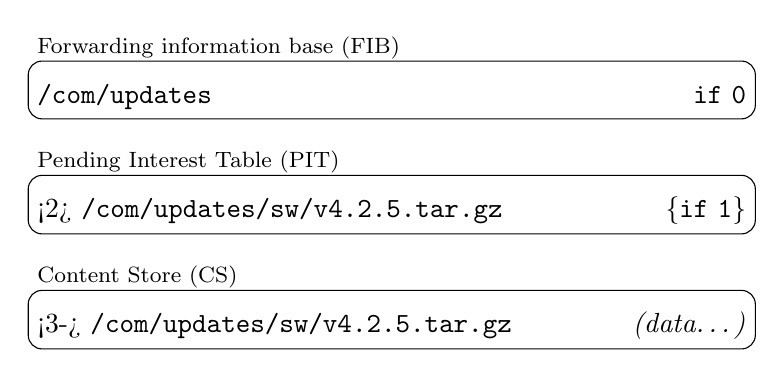
\begin{tikzpicture}
        \tikzset{datastructure/.style={rounded corners=5pt, draw, text width=9cm}}
        \node [datastructure] (FIB) {
          \\[0pt]
          \monobig{/com/updates} \hfill \monobig{if 0}
        };
        \node [above right=0pt of FIB.north west, yshift=-3pt] {\footnotesize Forwarding information base (FIB)};
        \node [datastructure] (PIT) [below=2em of FIB] {
          \\[0pt]
          {\uncover<2>{
            \monobig{/com/updates/sw/v4.2.5.tar.gz} \hfill \monobig{\{if 1\}}
          }}
        };
        \node [above right=0pt of PIT.north west, yshift=-3pt] {\footnotesize Pending Interest Table (PIT)};
        \node [datastructure] (CS) [below=2em of PIT] {
          \\[0pt]
          {\uncover<3->{
            \monobig{/com/updates/sw/v4.2.5.tar.gz} \hfill \textit{(data\dots)}
          }}
        };
      \node [above right=0pt of CS.north west, yshift=-3pt] {\footnotesize Content Store (CS)};
      \end{tikzpicture}
    }
  \end{columns}
\end{frame}

\subsection{Pending Interest Table redesign}
\begin{frame}[fragile]
  \frametitle{Pending Interest Table redesign I}
  PIT entries need an expiration time, for packets lost ``upstream''
  \vspace{-6pt}
  \begin{itemize}
    \item With a $1 s$ time-to-live: at least $5.5$ millions entries ($528 MB$)
  \end{itemize}
  Original design:
  \vspace{-6pt}
  \begin{itemize}
    \item Implemented as a hash table and a ring
    \item Require to periodically \emph{purge} expired entries from the bottom
      \uncover<2->{
        \begin{itemize}
          \item Cleaning up took up to $10 ms$ (routing one pkt: about $800 ns$)
          \item About $55000$ consecutive packets may go lost during purging
        \end{itemize}
      }
  \end{itemize}
  \vspace{-18pt}
  \begin{center}
    \includegraphics[width=.70\linewidth]{img/old_pit_sketch_trans.png}
  \end{center}

  \begin{comment}
  \begin{itemize}
    \item Implemented as a hash table and a ring
      \begin{itemize}
        \item The hash table only stores pointers to the ring, to keep it small
        \item Entries are timestamped: when stale, they must be purged
        \item Purging is currently performed online
      \end{itemize}
    \item With a time-to-live of $1 s$, at $5.5 Mpps$: at least $5.5$ millions entries ($528 MB$)
    \item A single expiring entry can linger at the bottom for $1 s$ causing the ring to fill up
    \item Cleaning up the whole buffer takes in the order of $10 ms$
      \begin{itemize}
        \item For comparison, routing a single packet takes about $800 ns$
        \item About $55000$ consecutive packets may go lost during purging
      \end{itemize}
    \item What remedies?
      \begin{itemize}
        \item Current hack: limit the number of packets purged in a raw (increasing the size accordingly)
        \item Use a plain hash table (less cache-friendly)?
        \item Asynchronous purge, with lock-free synchronization (single producer, single consumer)?
      \end{itemize}
  \end{itemize}
  \end{comment}
\end{frame}

\begin{frame}[fragile]
  \frametitle{Pending Interest Table redesign II}
  New design:
  \vspace{-6pt}
  \begin{itemize}
    \item Single hash table (more wasted memory)
    \item Follows same design principle (minimize accesses to RAM)
    \item Does not require any purging procedure
  \end{itemize}
  \vspace{-14pt}
  \begin{center}
    \includegraphics[width=\linewidth]{img/new_pit_sketch_trans.png}
  \end{center}
\end{frame}

\section{Performance evaluation}

\begin{frame}[fragile]
  \frametitle{Experimental setup}
  \begin{itemize}
    \item Two twin machines, each with two 10Gbps Ethernet ports
    \item Throughput is measured at the level of Ethernet payload
  \end{itemize}
  Initial assumptions:
  \begin{itemize}
    \item All names have the same length (three components)
    \item Every interest packet has a unique name: no CS hits
    \item The FIB contains one entry of length 1 matching all interests
  \end{itemize}
  \vspace{.5em}
  \begin{columns}
    \column{.6\linewidth}
    \resizebox{\linewidth}{!}{%
      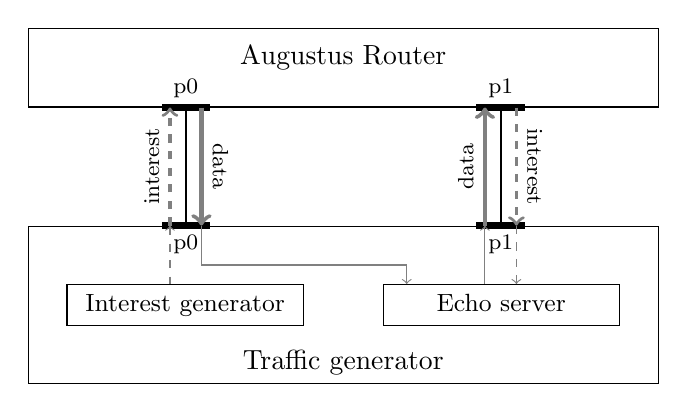
\begin{tikzpicture}

  \tikzset{cable/.style={thick}}
  \tikzset{dataline/.style={draw=black!50,ultra thick,->}}
  \tikzset{intline/.style={dashed,draw=black!50,very thick,->}}


  % Basic nodes

  \node [rectangle,draw=black,minimum width=8cm,minimum height=1cm]
    (augustus) {};
  \node [below=1mm of augustus.north] {Augustus Router};
  \node [rectangle,draw=black,minimum width=8cm,minimum height=2cm]
    (pktgen) [below=1.5cm of augustus] {};
  \node [above=0 of pktgen.south] {Traffic generator};
  \node [rectangle,draw=black,minimum width=3cm]
    (intgen) [left=5mm of pktgen.center] {\small Interest generator};
  \node [rectangle,draw=black,minimum width=3cm]
    (echoserver) [right=5mm of pktgen.center] {\small Echo server\vphantom{g}}; % phantom g to align boxes

  % Ports

  \newcommand\port[1]{ \draw #1 +(-3mm,-1pt) rectangle +(3mm,1pt) [fill]}

  \coordinate (augustus p0) at ([xshift=-2cm]augustus.south);
  \coordinate (augustus p1) at ([xshift=2cm]augustus.south);
  \coordinate (pktgen p0) at ([xshift=-2cm]pktgen.north);
  \coordinate (pktgen p1) at ([xshift=2cm]pktgen.north);

  \port{(augustus p0)};
  \port{(augustus p1)};
  \port{(pktgen p0)};
  \port{(pktgen p1)};

  \coordinate (augustus p0 int) at ([xshift=-.2cm]augustus p0);
  \coordinate (augustus p0 data) at ([xshift=.2cm]augustus p0);
  \coordinate (augustus p1 int) at ([xshift=.2cm]augustus p1);
  \coordinate (augustus p1 data) at ([xshift=-.2cm]augustus p1);
  \coordinate (pktgen p0 int) at ([xshift=-.2cm]pktgen p0);
  \coordinate (pktgen p0 data) at ([xshift=.2cm]pktgen p0);
  \coordinate (pktgen p1 int) at ([xshift=.2cm]pktgen p1);
  \coordinate (pktgen p1 data) at ([xshift=-.2cm]pktgen p1);

  % Port-to-port connections

  \node at (augustus p0.north) [anchor=south] {\footnotesize{p0}};
  \node at (augustus p1.north) [anchor=south] {\footnotesize{p1}};
  \node at (pktgen p0.south) [anchor=north] {\footnotesize{p0}};
  \node at (pktgen p1.south) [anchor=north] {\footnotesize{p1}};

  \draw [cable] (augustus p0) -- (pktgen p0);
  \draw [cable] (augustus p1) -- (pktgen p1);

  \draw [intline] (pktgen p0 int) -- (augustus p0 int)
    node [midway, above, sloped] {\footnotesize{interest}};
  \draw [intline] (augustus p1 int) -- (pktgen p1 int)
    node [midway, above, sloped] {\footnotesize{interest}};

  \draw [dataline] (pktgen p1 data) -- (augustus p1 data)
    node [midway, above, sloped] {\footnotesize{data}};
  \draw [dataline] (augustus p0 data) -- (pktgen p0 data)
    node [midway, above, sloped] {\footnotesize{data}};

  % Intra traffic generator connections

  \draw [intline,thin,<-] (pktgen p0 int) -- (pktgen p0 int |- intgen.north);
  \draw [dataline,thin] (pktgen p0 data) -- +(0,-5mm) -| ([xshift=-1.2cm]echoserver.north);
  \draw [intline,thin] (pktgen p1 int) -- (pktgen p1 int |- echoserver.north);
  \draw [dataline,thin,<-] (pktgen p1 data) -- (pktgen p1 data |- echoserver.north);

\end{tikzpicture}

    }
    \column{.4\linewidth}
    \frame{\includegraphics[width=\linewidth]{img/servers_back.jpg}}
    %\caption{Experimental setup}
  \end{columns}
\end{frame}


\subsection{Traffic generator}
\begin{frame}[fragile]
  \frametitle{Traffic generator}
  Evaluating performance of the packet generator alone, with a loop cable connecting the two ports on a single server
  \begin{figure}
    \includegraphics[height=.65\textheight]{img/traffgen_increasing_len.pdf}
    %\caption{Evaluating performance of the packet generator alone, with a loop cable connecting the two ports on a single server}
  \end{figure}
\end{frame}

\subsection{Evaluation of the new PIT design}
\begin{frame}[fragile]
  \frametitle{Evaluation of the new PIT design}

  \begin{columns}[c]
    \column{.35\textwidth}
    \begin{figure}
      \includegraphics[width=\textwidth]{img/pit_thr_cmp.pdf}
    \end{figure}
    \column{.65\textwidth}
    \begin{figure}
      \includegraphics[width=.85\textwidth]{img/augustus_load_loss.pdf}
    \end{figure}
  \end{columns}

  Considering throughput, performance does not decrease\\
  Working close to overload condition, loss decreases considerably

\end{frame}

\subsection{Router performance}

\begin{frame}[fragile]
  \frametitle{Router performance over packet size: single-core}
  
  \includegraphics[width=\textwidth]{img/augustus_increasing_len_0x1.pdf}
\end{frame}

\begin{frame}[fragile]
  \frametitle{Router performance: threads and core mapping I}
  DPDK requires to pin threads to processing cores\\
  Test servers: 2 sockets $\times$ 8 cores $\times$ 2 (hyperthreading)

  \begin{figure}
    \includegraphics[height=.7\textheight]{img/cpus_horiz.pdf}
  \end{figure}
\end{frame}

\begin{frame}[fragile]
  \frametitle{Router performance: threads and core mapping II}
  \begin{columns}[c,onlytextwidth]
    \column{0.6\textwidth}
    \setcounter{beamerpauses}{2}
    \begin{tikzpicture}
      \node [inner sep=0pt] (plot)
        {\includegraphics[width=\linewidth]{img/augustus_multithread_slim.pdf}};
      \begin{scope}[
          shift=(plot.south west),
          x={(plot.south east)},y={(plot.north west)}
        ]
        %\draw [thick,red] (0,0) -- (0,1) -- (1,1) -- (1,0) -- cycle;
        \coordinate (origin) at (.209,.141);
        \coordinate [right=.077 of origin] (onezero);
        \coordinate [above=.132 of origin] (zeroone);
        \begin{scope}[shift=(origin), x={(onezero)}, y={(zeroone)}]
          \foreach \x/\y in {0/0, 0/1, 0/6, 1/0, 9/0, 0/6} {\draw [fill=yellow] (\x,0) circle (1pt);}
          \foreach \x/\y in {0/2.1, 1/2.6, 2/3.5, 3/3.8, 4/3.3, 5/5.8, 6/2.8, 7/5.5, 8/3.8, 9/3.6} {
            %\draw [fill=green] (\x,\y) circle (1pt);
            {\only<+|handout:0>{ \draw [<-,ultra thick,draw=black] (\x,\y) -- +(0,.5); }}
          }
        \end{scope}
      \end{scope}
    \end{tikzpicture}

    \column{0.4\textwidth}
    \setcounter{beamerpauses}{2}
    \begin{tikzpicture}
      \node [inner sep=0pt] (map)
        {\includegraphics[width=\linewidth]{img/cpus_horiz.pdf}};
      \begin{scope}[
          shift=(map.south west),
          x={(map.south east)},y={(map.north west)}
        ]
        \tikzset{corebox/.style={draw=red, fill=red, fill opacity=.3}}
        \newcommand\rect[2]{+(-#1,-#2) rectangle +(#1,#2)}
        \newcommand\coreboxrect{\rect{.020}{.02}}
        \newcommand\corebox[1]{\draw [corebox] (#1) \coreboxrect;}

        \def\l{.055}  % left column
        \def\r{.945}  % right column
        \def\t{.93}   % top row
        \def\h{.116}  % row height
        \def\hh{.045}  % vertical dist between two hw threads

        \coordinate (p0) at (\l,\t);
        \coordinate (p1) at (\r,\t);
        \coordinate (p14) at (\l,\t-7*\h);
        \coordinate (p16) at (\l,\t-\hh);

        {\only<+|handout:0>{ \corebox{p0} }}
        {\only<+|handout:0>{ \corebox{p0} \corebox{p16} }}
        {\only<+|handout:0>{ \corebox{p0} \corebox{p14} }}
        {\only<+|handout:0>{ \corebox{p0} \corebox{p1} }}
        {\only<+|handout:0>{
          \foreach \i in {0,2,4,6} { \corebox{\l,\t-\i*\h} }
        }}
        {\only<+|handout:0>{
          \foreach \i in {0,1} { \corebox{\l,\t-\i*\h} \corebox{\r,\t-\i*\h} }
        }}
        {\only<+|handout:0>{
          \foreach \i in {0,...,7} { \corebox{\l,\t-\i*\h} }
        }}
        {\only<+|handout:0>{
          \foreach \i in {0,1,2,3} { \corebox{\l,\t-\i*\h} \corebox{\r,\t-\i*\h} }
        }}
        {\only<+|handout:0>{
          \foreach \i in {0,...,7} { \corebox{\l,\t-\i*\h} \corebox{\r,\t-\i*\h} }
        }}
        {\only<+|handout:0>{
          \foreach \i in {0,...,7} { \corebox{\l,\t-\i*\h} \corebox{\r,\t-\i*\h} }
          \foreach \i in {0,...,7} { \corebox{\l,\t-\i*\h-\hh} \corebox{\r,\t-\i*\h-\hh} }
        }}
      \end{scope}
    \end{tikzpicture}
  \end{columns}
\end{frame}

\begin{frame}[fragile]
  \frametitle{Router performance over packet size: multi-core}
  
  \includegraphics[width=\textwidth]{img/augustus_increasing_len_0xF.pdf}
\end{frame}

\section{Conclusions and future work}
\begin{frame}[fragile]
  \frametitle{Conclusions and future work}
  \begin{itemize}
    \item The redesigned PIT improved performance under TODO.
    \item The router reached $5.4$ Mpps, reaching line rate with packets of $220$ bytes ($\sim180$ bytes application-level payload), showing the feasibility of deploying a CCN router on current hardware
    \item Configuration and deployment must be hardware aware: no software/hardware decoupling for high-performance routing
  \end{itemize}
%\end{frame}
%\begin{frame}[fragile]
%  \frametitle{Missing bits}

  \onslide<+->
  \onslide<+->
  Missing bits:

  \begin{itemize}
    \item How does it scale with FIB size?
    \item So far, the local cache was just a burden (kept up-to-date, but any lookup fails): what improvements could we get with web-like traffic?
    \item A port of the software as a module for the \emph{Click} router is in progress: what's the impact on performance?
  \end{itemize}
\end{frame}


% copying some code from the \plain command, adding <handout:0>
%\plain<handout:0>{% .........
\begingroup
\setbeamercolor{background canvas}{
  use=palette primary,
  parent=palette primary
}
\begin{frame}<handout:0>[plain,c,fragile]
  \begin{center}
    \usebeamercolor[fg]{palette primary}
    \usebeamerfont{section title}
    {\large \inserttitle}

    \vspace{1em}

    {\normalsize Thanks for your attention}
  \end{center}
\end{frame}
\endgroup

\extraslidesbegin

\section*{bibliography}
\begin{frame}[allowframebreaks]
  \frametitle{References}

  \setbeamertemplate{bibliography item}[text]
  \bibliography{davide_kirchner_thesis_pres}
  \bibliographystyle{alpha}
\end{frame}


\section*{Lost slides}
\begin{frame}[fragile]
  \frametitle{Click interface -- \textit{in progress}}
  \verbatiminput{extra/icnrouter.click.txt}
\end{frame}

\begin{frame}[fragile]
  \frametitle{Routing in CCN - Interest packets}
  \begin{algorithm}[H]
    \DontPrintSemicolon
    \KwIn{$p$: CCN interest packet}
    \If{$p.name \in ContentStore.names()$}{
  $nexthop := p.source\_hop$\;
  $nexthop.send(ContentStore.get\_data(p.name))$\;
}
\ElseIf{$p.name \in PendingInterestTable.names()$}{
  $PendingInterestTable.aggregate\_entry(p.name)$\;
}
\ElseIf{$any\ prefix\ of\ p.name\ matches\ ForwardingInfoBase$}{
  $nexthop := ForwardingInfoBase.longestPrefixMatch(p.name)$\;
  $nexthop.send(p)$\;
}
\Else{
  \tcp{Drop}
}

    %\caption{\textsc{CCN interest route}}
  \end{algorithm}
\end{frame}

\begin{frame}[fragile]
  \frametitle{Routing in CCN - Data packets}
  \begin{algorithm}[H]
    \DontPrintSemicolon
    \KwIn{$p$: CCN data packet}
    $ContentStore.store(p)$\;
\If{$p.name \in PendingInterestTable.names()$}{
  $nexthops := PendingInterestTable.remove(p.name)$\;
  \ForEach{$nexthop \in nexthops$}{
    $nexthop.send(p)$\;
  }
}
\Else{
  \tcp{Drop}
}

    %\caption{\textsc{CCN data route}}
  \end{algorithm}
\end{frame}

\begin{frame}[fragile]
  \frametitle{Pending Interest Table redesign}
  PIT entries need an expiration time, for packets lost ``upstream''
  \vspace{-6pt}
  \begin{itemize}
    \item With a $1 s$ time-to-live: at least $5.5$ millions entries ($528 MB$)
  \end{itemize}
  Original design:
  \vspace{-1.2cm}
  \begin{flushright}
    \includegraphics[width=.7\linewidth]{img/old_pit_sketch_trans.png}
  \end{flushright}
  \vspace{-2.7cm}
  \begin{columns}[t]
    \column{.5\linewidth}
    \begin{lstlisting}[language=c,escapechar=\%]
struct orig_pit_ring_entry {
 bool active;
 uint64_t expiry;
 uint64_t nonce_bf;
 char full_name[MAX_NAME_LEN];
 uint64_t interface_bitmask;
 // index in HT for cleanup
 uint32_t bucket_index;
 uint8_t tab_in_bucket;
};
    \end{lstlisting}
    \column{.5\linewidth}
    \begin{lstlisting}[language=c,escapechar=\%]
%\\%
%\\%
%\\%
%\\%
%\\%
struct orig_pit_ht_entry {
 bool busy;
 uint32_t crc;
 uint32_t ring_index;
};
    \end{lstlisting}
  \end{columns}
\end{frame}

\extraslidesend

\end{document}

              
